\documentclass{beamer}
\usepackage[utf8]{inputenc}
\usepackage{graphicx}
\usepackage{color}
%\usetheme{Hannover}
\newcommand{\hilight}[1]{\textbf{\textcolor{structure.fg!85}{#1}}}
\setbeamertemplate{footline}[frame number]

\usepackage{hyperref}
\hypersetup{
    colorlinks=true,
    linkcolor=blue,
    filecolor=magenta,      
    urlcolor=cyan,
}

\author[Sowmya Vajjala]{Sowmya Vajjala}

\title[SfSNLP]{NLP without Annotated Dataset}
\subtitle{Generate your labeled data}


\date{15 January 2021}

\institute{Seminar f\"ur Sprachwissenschaft, University of T\"ubingen, Germany}
%%%%%%%%%%%%%%%%%%%%%%%%%%%

\begin{document}

\begin{frame}\titlepage
\end{frame}

\begin{frame}
\frametitle{Class Outline}
\begin{itemize}
    \item Quick recap of last class
    \item Anonymization of data in NLP 
    \item Generating your own data
        \begin{itemize}
    \item Weak supervision: An overview
    \item Automatic Data Labeling: Some examples
    \item Data Augmentation: Some examples
    \item Text classification: An overview
    \end{itemize}
-(How all these come together: on Monday)
\end{itemize}
\end{frame}

\begin{frame}
\frametitle{General Housekeeping Stuff}
\begin{itemize}
    \item Teams/Papers: I posted teams info on the forum.
    \item Presentation schedule  (also posted on forum)
    \begin{enumerate}
        \item 22nd January: Teams 1--3
        \item 25th January: Teams 4--7
        \item 27th January: Teams 7--9
    \end{enumerate}
    \item Format: 15-20 minutes of presentation, Around 10 min of discussion per team (everyone can ask questions. Presenters don't have to know all answers. I will also try to answer some of the questions that come up!)
\end{itemize}
\end{frame}

\begin{frame}
\frametitle{Quick Recap of Last Class}
\begin{itemize}
    \item Corpus collection: different ways of using existing datasets, collecting our own data, generating data.
    \item Text extraction: from different file formats
    \item Corpus Exploration: understanding some basic characteristics of the corpus
\end{itemize}
-Any questions on this part?
\end{frame}

\begin{frame}
\frametitle{Anonymization in NLP discussion}
\begin{itemize}
    \item Why? : When sharing a sensitive dataset publicly (or even privately), we should not be compromising the identity of people in it. 
\pause \item How?: using NER to replace some categories (people names, organizations etc) - name replaced with another name etc. 
\pause \item However, it is not always a NE. Take this sentence: \textit{John Brown, the long jump record holder, retired yesterday.} - "the long jump record holder" can reveal the identity of the person here. \pause
\item Something like a username may not be identified as a NE, but is sensitive information in most contexts. 
\item NER is objective. Anonymization is subjective (what entity should be anonymized in this particular context?)
\end{itemize}
(\href{http://www.lrec-conf.org/proceedings/lrec2006/pdf/200_pdf.pdf}{Source})
\end{frame}

\begin{frame}
\frametitle{Some example scenarios where anonymization is done}
\begin{itemize}
    \item Clinical data - names of patients/doctors, phone numbers, addresses etc. 
    \item Social media data - may be twitter handles?
    \item Information extraction from resume etc. - names of univs, past companies etc
    \item Personal legal/finance documents - names, addresses, phone numbers etc. 
\end{itemize}
\end{frame}

\begin{frame}{Challenges in anonymization}
    \begin{itemize}
    \item The categories that should be de-identified are usually also the ones important for performing NLP tasks! So, if we replace an age group with another, will the system be just as effective?
\pause \item What should be replaced, not changed, or deleted? 
\pause \item Is it sufficient? -there are many instances of identifying individuals from anonymized data, by combining information from other sources. 
\end{itemize}
\end{frame}

%TODO!
\begin{frame}{What to do?}
\framesubtitle{Interesting work by \href{https://www.aclweb.org/anthology/2020.coling-main.32.pdf}{Volodina et.al., 2020}}
"Towards Privacy by Design in Learner Corpora Research: A Case of On-the-fly Pseudonymization of Swedish Learner Essays"
    \begin{itemize}
        \item  "In the absence of labeled pseudonymized data to apply dataintensive machine learning approaches, we choose to experiment with rule-based approaches to detect, label and pseudonymize information that we define as personal on a set of L2 Swedish essays.
\pause \item What is anonymized: license numbers, bank accounts, dob, email, phone etc.; ge0-data (address, country etc); person and institution names; and what they call: sensitive info (ethnicity, political/religious views etc).
\pause \item How?: NER, regular expressions, rules, pos tagging + rules etc. 
    \end{itemize}
\end{frame}

\begin{frame}{Some resources/code}
    \begin{itemize}
        \item \href{https://pypi.org/project/cdeid/}{cdeid - de-identification library}
        \item \href{https://github.com/microsoft/presidio}{Presidio - free and open-source tool from Microsoft}
        \item \href{https://github.com/Planeshifter/deidentify}{A de-identification tool with a UI}
        \item \href{https://github.com/nedap/deidentify}{Dutch de-identification software + paper}
        \item \href{https://pii-tools.com/}{PII-Tools} (proprietary)
    \end{itemize}
\end{frame}

\begin{frame}{Some references}
Links to some recent research in this direction:
    \begin{itemize}
        \item \href{https://sites.google.com/view/wsdm-privatenlp-2020}{Private NLP workshop}
        \item \href{https://www.aclweb.org/anthology/D18-1001/}{Privacy-preserving Neural Representations of Text} (2018 research paper)
        \item \href{https://towardsdatascience.com/perfectly-privacy-preserving-ai-c14698f322f5}{Perfectly Privacy Preserving AI} by Patricia Thaine (2020)
        \item \href{https://www.amazon.science/blog/preserving-privacy-in-analyses-of-textual-data}{Preserving Privacy in Analysis of Textual Data} - from Amazon. 
    \end{itemize}
\end{frame}

\begin{frame}
\frametitle{A small exercise about datasets and their issues}
Time 20 minutes, in breakout rooms.

Go to Linguistic Data Consortium's Top-10 most distributed NLP corpora (https://catalog.ldc.upenn.edu/topten). Pick any corpus you want. See if you can build a datasheet for this dataset (Look at the full list of questions at the end of \href{http://www.fatml.org/media/documents/datasheets_for_datasets.pdf}{"Datasheets for Datasets", Gebru et.al., 2018}). 

One person per team will summarize their observations at the end. Don't do exhaustively, do what you can easily understand from available material. 
\end{frame}

\begin{frame}
\frametitle{}
Summarize your findings + Any questions you want to ask. 
\end{frame}

\begin{frame}
\frametitle{}
Let us may be break for 5 minutes, before we start with automatic data labeling!
\end{frame}


\begin{frame}
\frametitle{Weak Supervision: An Introduction}
\begin{itemize}
    \item Generally, most 'learning' methods used in NLP are data hungry. However, it is time consuming and also expensive to hand label so much of data for each new problem. \pause
    \item Sometimes, we may have to update existing labels to suit changed guidelines or just update the dataset etc. (not so uncommon in real world). How do we handle the costs/time taken? \pause
    \item "Weak supervision" refers to a machine learning approach which relies on "imprecise" training data, which is potentially "generated" automatically. \pause
    \item An approach: write code based on observed patterns in data to label subsets of unlabeled data.
    \item ... and then use this code to create labeled training data for our ML model
\end{itemize}
\end{frame}

\begin{frame}
\frametitle{Weak Supervision: Continued}
\begin{itemize}
    \item Clearly, this is a noisy dataset. There may be labeling errors. What now? \pause
    \item Snorkel's approach: \\ 
\begin{itemize}
    \item Create a noisy training set through "labeling functions" (I showed one in the last class.)
    \item Learn a model of this noise (to understand which of these functions are good in terms of labeling)
    \item Uses this model to train a more powerful model which learns from the noise. 
\end{itemize}
\end{itemize}
The next few slides will rely on \href{https://db.cs.washington.edu/events/workshop/2019/slides/alex-ratner.pdf}{This talk slides by Alex Ratner, one of the people behind Snorkel.}
\end{frame}

\begin{frame}{}
    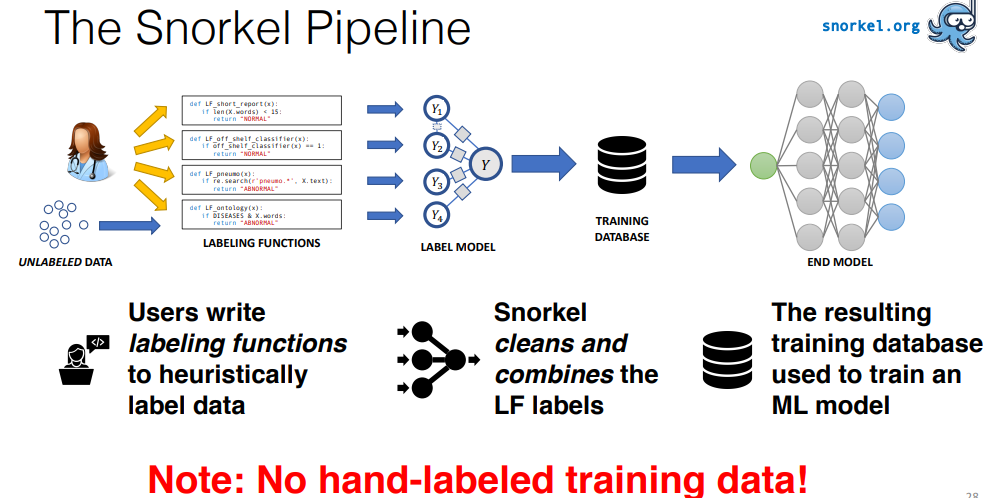
\includegraphics[width=\textwidth]{figures/snorkelradiologyexample.PNG}
    
\href{Source}{https://db.cs.washington.edu/events/workshop/2019/slides/alex-ratner.pdf}
\end{frame}

\begin{frame}{When is this useful?}
    \begin{itemize}
        \item No training data
        \item Expensive training data (which needs specific expertise)
        \item Private data (which can't be exposed to crowd workers, for example)
        \item Constantly changing data
    \end{itemize}
\end{frame}

\begin{frame}
\frametitle{How to "create" data?}
    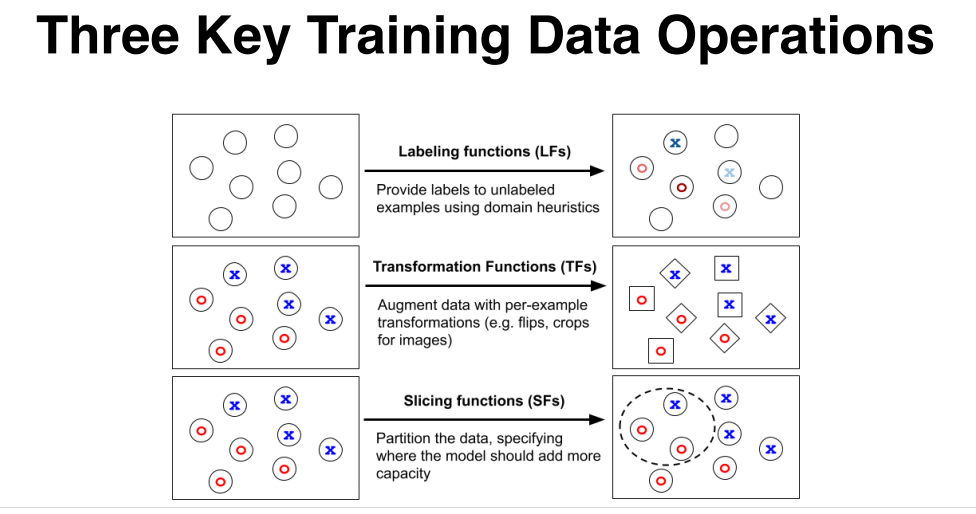
\includegraphics[width=\textwidth]{figures/3snorkelops.PNG}
\end{frame}

\begin{frame}
\frametitle{How to "create" data?- Labeling Functions}
    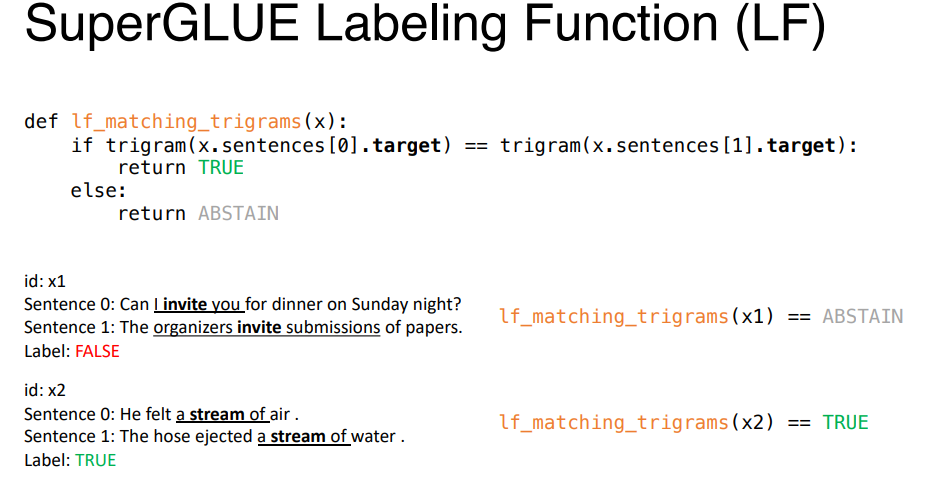
\includegraphics[width=\textwidth]{figures/lfexample.PNG}
\end{frame}

\begin{frame}
\frametitle{How to "create" data? - augmentation}
    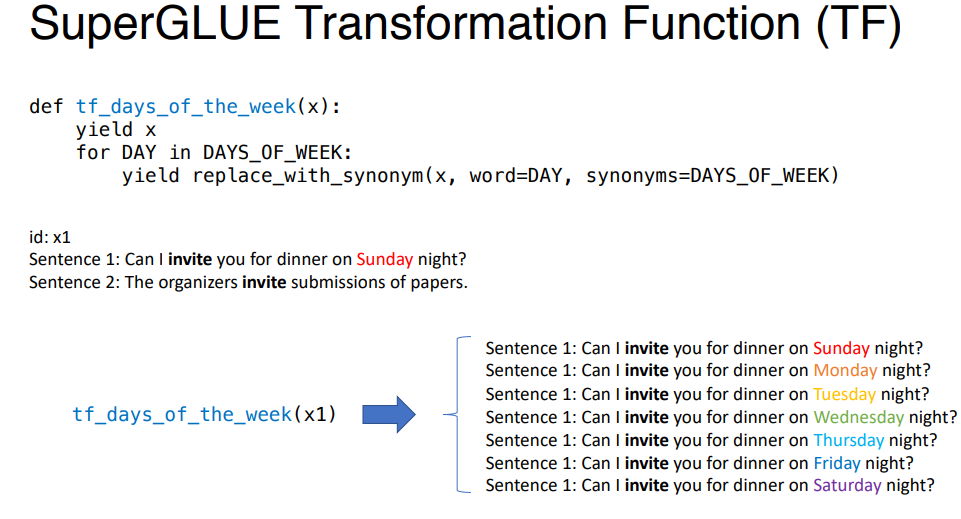
\includegraphics[width=\textwidth]{figures/tfexample.PNG}
\end{frame}

\begin{frame}
\frametitle{How to "create" data? - slicing}
    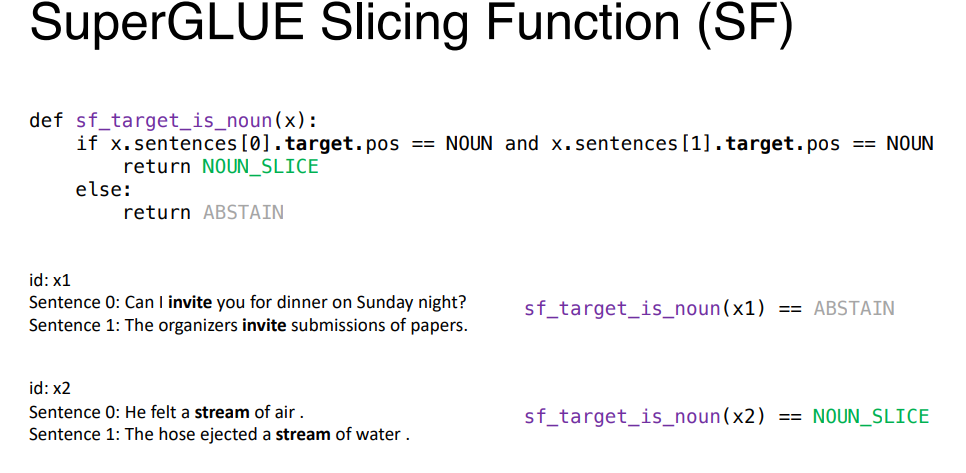
\includegraphics[width=\textwidth]{figures/slicingexample.PNG}
\end{frame}

\begin{frame}
\frametitle{What is "slicing"?}
\begin{itemize}
    \item In real-world systems, some predictions/categories may be more important than others.
    \item However, when we build these learning models, we look at overall performance.
    \item So, "slicing" functions in Snorkel identify these subsets of data that we should particularly care about. 
    \item Note: This is done after training data is ready, otherwise we cannot create these subsets!
\end{itemize}
an interesting tidbit: slice based learning was deployed in production systems at Apple in 2019. 
\end{frame}

\begin{frame}
\frametitle{Let us revisit the snorkel approach}
    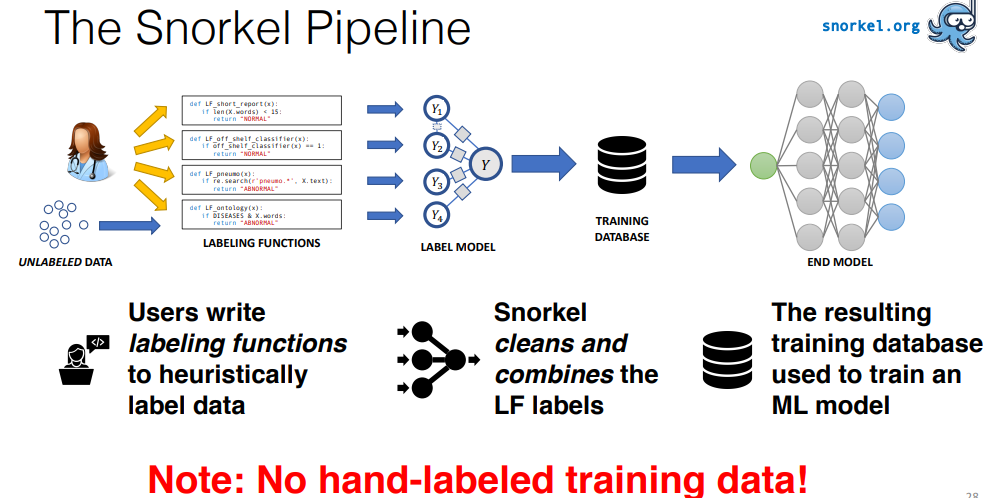
\includegraphics[width=\textwidth]{figures/snorkelradiologyexample.PNG}
\end{frame}

\begin{frame}{What is happening at "Label model"?}
There is actually no "labeled" data. What is this "label model" learning? and how? \pause

\bigskip

Key idea: learn from the agreements and disagreements among label functions about a single data point!
\end{frame}

\begin{frame}{It all sounds good, does this really work?}
\framesubtitle{Snorkel in Real world (2019)}
    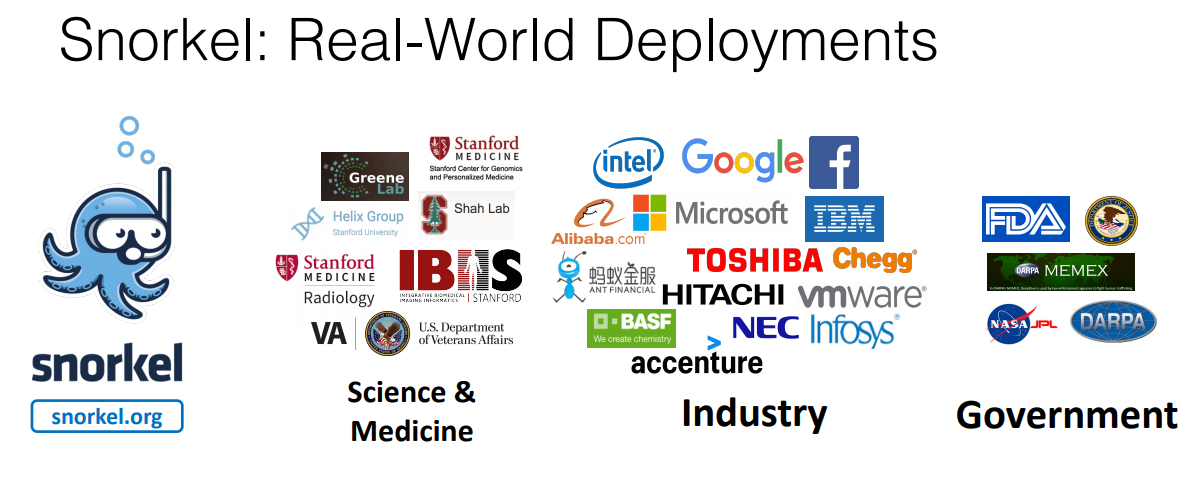
\includegraphics[width=\textwidth]{figures/snorkelrealworld.PNG}
    \href{Source}{https://db.cs.washington.edu/events/workshop/2019/slides/alex-ratner.pdf}
\end{frame}

\begin{frame}
\frametitle{Specific Examples - Industry Usecases}
    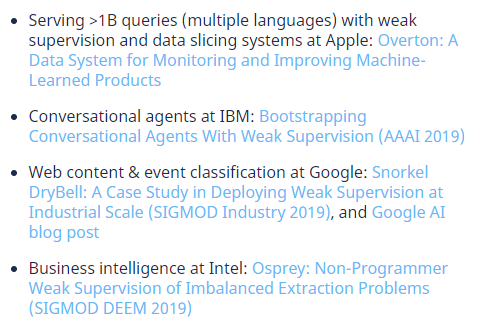
\includegraphics[width=\textwidth]{figures/snorkelusepapers.PNG}
\end{frame}

\begin{frame}
\frametitle{Specific Examples - Clinical NLP}
    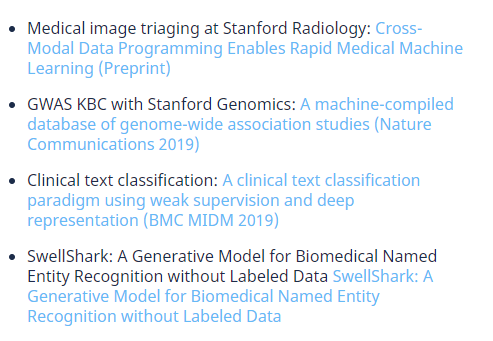
\includegraphics[width=\textwidth]{figures/snorkelclinicalnp.PNG}
\end{frame}

%TODO: An exercise - perhaps take a paper and ask students to go through the data creation part?? 
\begin{frame}{}
    But, how does this whole developing labeling functions, transformations etc work?? How should we look for patterns?
\end{frame}

\begin{frame}{Let us find out}
\framesubtitle{Time for an exercise}
    \href{https://docs.google.com/spreadsheets/d/1ESW1FQ36rSxFww3jo7IuAzw7HPq4_MATY9-hRhX6CnE/edit?usp=sharing}{Here} is a spreadsheet with some sentences. They are to be labeled as positive/negative/neutral sentiment, from the perspective of a investor. So, your task is to see if you can come up with some patterns to "label" this data.
    
    Estimated time: May be around 20 minutes. 
\end{frame}

\begin{frame}{}
    Your observations, 1 person per team can summarize.
    
    Data source: \url{https://www.kaggle.com/ankurzing/sentiment-analysis-for-financial-news}
\end{frame}

\begin{frame}
\frametitle{Snorkel Approach: A summary}
\begin{itemize}
    \item We may frequently see situations without training data.
    \item It is possible to generate training data through heuristics (string matching, regex etc), and a few "tricks" (like augmentation)
    \item Not all training instances are equally important. So, we can partition the data (slicing) and identify critical subsets.
    \item This is a two stage "modeling" - one for consolidating all labeling functions to build a training set, one for learning from this training set. 
\end{itemize}
\end{frame}
    
\begin{frame}{You talked about a lot of stuff}
    \framesubtitle{How do we actually "DO" this?}
    \begin{itemize}
        \item Monday - I thought this overview is important before showing a working code example!
        \item Source: "Spam classification" tutorial from Snorkel, but hopefully with some additions based on corpus exploration \pause
        \item But I keep saying "classification". What is it? How does it work?
        \item and Why classification? Why not machine translation or some other task? 
    \end{itemize}
\end{frame}
%3-4 slides on :Is this useful? where is it already being used?:

\begin{frame}
\frametitle{}
Let us may be break for 5 minutes, before we start with text classification!
\end{frame}


\begin{frame}
\frametitle{Text Classification}
\begin{itemize}
    \item It is the task of assigning one (or more) categories to a given piece of text from a larger set of possible categories. \pause
    \item  In the email spam–identifier example, we have two categories—spam and non-spam—and each incoming email is assigned to one of these categories. \pause
    \item This task of categorizing texts based on some properties has a wide range of applications across diverse domains \pause
    \item Consider a scenario where we want to classify all reviews for a product into three categories: positive, negative, and neutral. 
    \item The challenge here is to “learn” this categorization from a collection of examples and predict the categories for new, unseen products and new customer reviews.
\end{itemize}
\end{frame}

\begin{frame}{Text Classification Pipeline}
    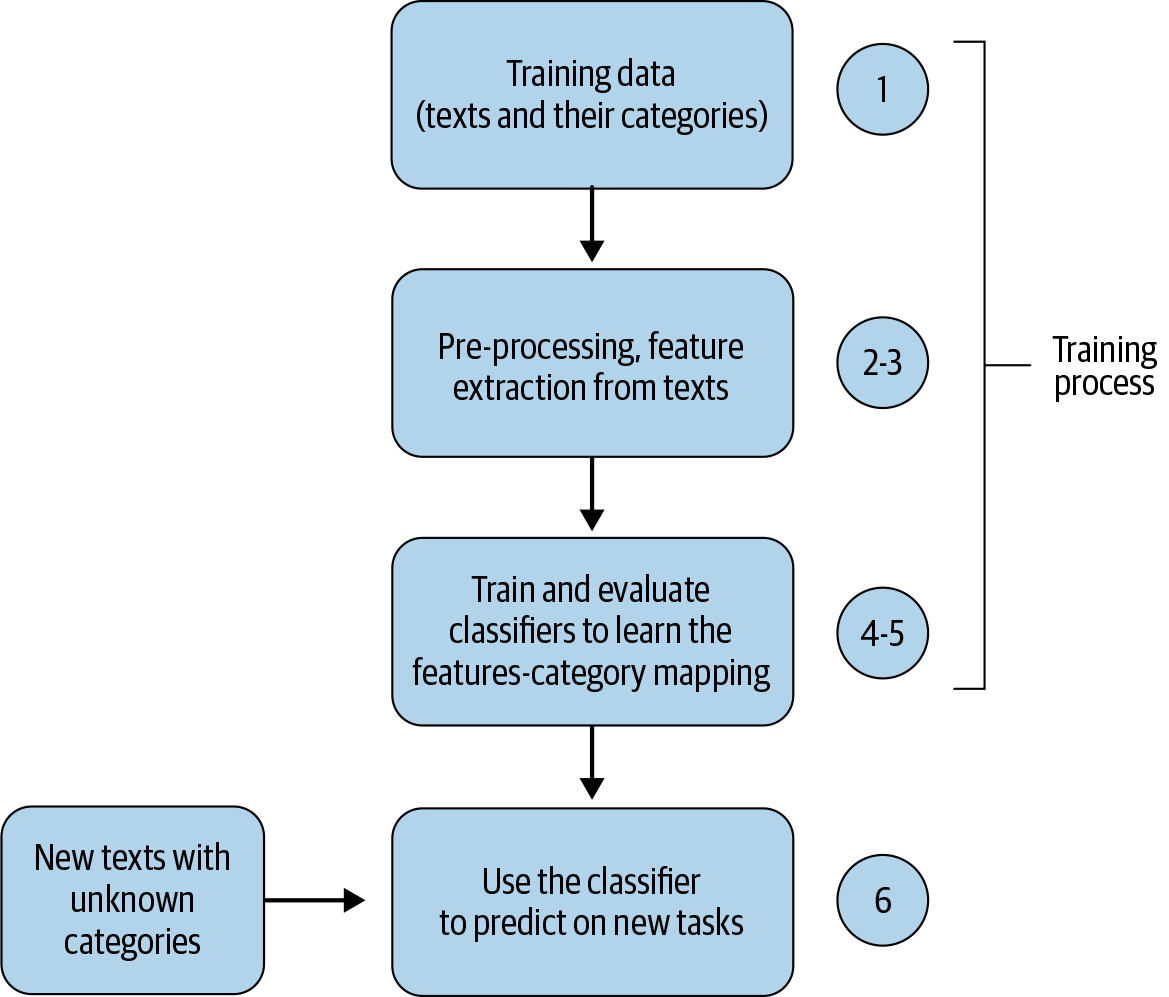
\includegraphics[width=0.8\textwidth]{figures/tcpipeline.png}
    source: Practical NLP book
\end{frame}

\begin{frame}{Text Classification Pipeline}
    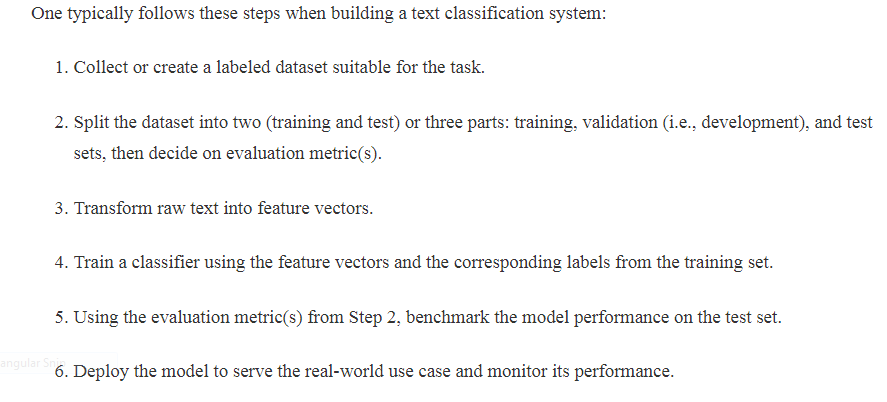
\includegraphics[width=\textwidth]{figures/tcsteps.png}
        source: Practical NLP book
\end{frame}

\begin{frame}
\frametitle{Text Classification Pipeline}
\begin{itemize}
    \item So, we talked about how to acquire or create our own training data.
    \item We also talked about pre-processing of text, and feature extraction to some extent.
    \item I showed an example of how to develop a sentiment classifier and use it to make predictions on new text.
    \item But what is happening during the "development" phase of a classifier? 
\end{itemize}
\end{frame}

\begin{frame}
\frametitle{Some commonly used features in text classification}
\begin{itemize}
\item ngrams (word, character, POS, mixed representations)
\item neural embeddings (word, character, sentence, document embeddings)
\item specific hand-crafted features: e.g., number of spelling errors, number of dependent clauses per clause, number of preposition phrases per sentence etc.
\item feature representation: binary (presence or absence), count (number of occurrences), ratios etc.
\end{itemize}
\end{frame}

\begin{frame}
\frametitle{Some commonly used learning algorithms}
\begin{itemize}
\item Naive bayes classifier
\item K-nearest neighbors classifier
\item Logistic regression
\item Decision trees
\item Random forests
\item Support vector machines
\item neural network classifiers
\end{itemize}
.. etc. \\ Note: I will only give an overview of how these work. Details are found in machine learning classes.
\end{frame}

\begin{frame}{Naive Bayes Classifier}
\begin{itemize}
\item Let us say I have a collection of emails (E1, E2 ... En). My problem is to classify them as spam or non-spam.
\item Let us assume I already have some training data of 1000 emails labeled as Spam, 1000 labeled non-spam.
\item Bayes classifier solves the text classification problem using bayes rule. For some email E1\\
P(spam$|$E1) = P(spam)*P(E1$|$spam)/P(E1) \\
P(non-spam$|$E1) = P(non-spam)*P(E1$|$non-spam)/P(E1) 
\item if first probability is higher than second, the email is spam. Else, it is non-spam.
\item Since this is a comparison, we can ignore the denominator.
\end{itemize}
\end{frame}
    
\begin{frame}
\frametitle{Naive Bayes - continued}
Let us take individual terms:
\begin{itemize}
\item P(spam), P(non-spam): prior probability of seeing a spam or non-spam message. If your training data has 400 spam and 100 non-spam messages, what are P(spam) and P(non-spam)? \pause
\item P(E1$|$spam),P(E1$|$non-spam): likelihood that the email is actually spam or non-spam based on our training data. How do we get this?
\item If we take a "bag of words" approach, and consider each word as a feature, each unique word in the email becomes a feature. 
\item If an email has only two words: "my mail", P(E1$|$spam) = P(my$|$spam)*P(mail$|$spam). P(E1$|$non-spam) = P(my$|$non-spam)*P(mail$|$non-spam). \pause
\item If an email has 100 words, P(E1$|$spam) and P(E1$|$non-spam) are products of 100 conditional probabilities. You assign E1 to spam if P(E1$|$spam) is higher than P(E1$|$non-spam) and vice-versa.
\end{itemize}
\end{frame}

\begin{frame}
\frametitle{Naive Bayes - conclusion}
\begin{itemize}
\item Assumption: Each feature is independent of the other.
\item There is no in-built way to account for inter-correlation between features
\item So, this assumption does not really tell the whole story about what is happening. But it works for predictive modeling! 
\end{itemize}
\end{frame}

\begin{frame}
\frametitle{k-NN classifier}
\begin{itemize}
\item Idea: A document belongs to the majority category among its k-neighbors. \pause
\item Let us say my classification problem is: classifying movie reviews into three groups - positive, negative, neutral.
\item My training data: say 500 examples for each of these categories.
\item Let us say I am using only two features: Use of positive adjectives, Use of negative adjectives 
\item If I say my k is 5, when I have to classify a new review, and 3 of its neighbors on this feature space have category "positive", 1 has "negative", 1 has "neutral", I will choose "positive" as the category for this new review, because majority of my k neighbors  have "positive".
\item What is neighborhood? - any measure of distance. 
\end{itemize}
\end{frame}

\begin{frame}
\frametitle{k-NN classifier - 2D example}
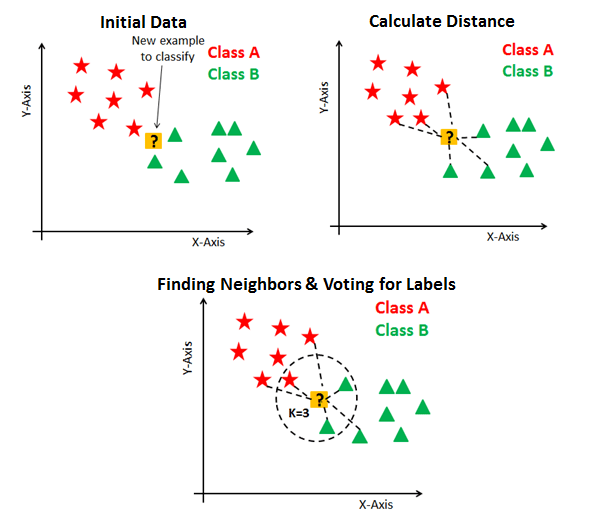
\includegraphics[width=0.9\textwidth]{figures/knnexample.png}
\\ \href{https://www.datacamp.com/community/tutorials/k-nearest-neighbor-classification-scikit-learn}{Source}
\end{frame}

\begin{frame}
\frametitle{kNN - conclusion}
\begin{itemize}
\item Also called "instance based classifier" or "lazy learner"
\item Does not really have a "model" or "function". All computation of near-ness or far-ness happens during actual classification
\item If you have large amounts of training data, and large feature set, this will become extremely slow. 
\item selecting k is heuristic.
\item relationship between features is till not considered. Features are considered independent of each other.
\end{itemize}
\end{frame}

\begin{frame}
\frametitle{Logistic Regression}
\begin{itemize}
\item Goal: same as any other classification algorithm. Classify a given text into one of the pre-defined categories, based on some feature representation.
\item Difference compared to naive bayes or knn: learning function.
\item Learning function in Logistic Regression:
\begin{enumerate}
\item If x is my text, f$_1$, f$_2$... f$_i$ is my feature vector for this text, C = {c1, c2, c3} are my three possible categories, \pause
\item for a class c,\\ p(c$|$x) = $\frac{exp(\sum_{i=1}^n (w_i*f_i(c,x))} {\sum_{c^\prime \in C} exp(\sum_{i=1}^n (w_i*f_i(c^\prime,x))}$
\item The class with the maximum probability in will be the predicted class. Since it is a comparison, again, we  can ignore denominator.
\end{enumerate}
\end{itemize}
\end{frame}

\begin{frame}{Logistic Regression}
    \begin{itemize}
        \item Note: You don't have to struggle with the math. There are ready to use implementations you can use if you want. 
        \item Check Chapter 5 in Jurafksy \& Martin for a detailed discussion on Logistic Regression (link in last slide)
        \item It is useful to know this, if you:
        \begin{itemize}
            \item Want to get into NLP research, work with deep learning etc.
            \item Work in a software company on NLP stuff: Logistic Regression is often the first baseline algorithm (and it can be a very strong one at that!)
        \end{itemize} \pause 
        \item (personal experience): At one point, I deployed a comment moderator for "The Globe \& Mail", Canada's largest news paper (2019 March). This was based on Bag of n-gram features + Logistic Regression!
    \end{itemize}
\end{frame}

\begin{frame}
\frametitle{Measuring Success of your classification approach}
Multiple ways. Depends on the nature of your dataset, and your application. Here are a few common measures:
\begin{itemize}
\item Prediction accuracy on test set: commonly used
\item False positive rate (Type 1 Error), False negatives (Type 2 error) 
\item Precision (TP/(TP+FP)), Recall (TP/(TP+FN)), F-score (2PR/(P+R))
\item Revenue increase - in e-commerce applications
\end{itemize}
,,, ,,,,
\end{frame}

\begin{frame}
\frametitle{Text Classification: Conclusion}
\begin{itemize} 
\item Many more algorithms. For NLP specific discussion, check out Jurafsky and Martin, 3rd Edition (Chapters 4,5, 7, 8, 9)
\item scikit-learn is a free machine learning library in Python that has implementations of several classification algorithms. 
\item spacy and huggingface support a lot of state of the art approaches for text classification (among others). 
\item I will show: examples with snorkel and scikit-learn (monday) and huggingface (wednesday). 
\end{itemize}
\end{frame}

\begin{frame}
\frametitle{Plan for the coming days}
\begin{itemize}
    \item Monday: Snorkel tutorial covering labeling functions, augmentation, slicing examples
   \\  (I am going to follow the tutorial on their website, with a few alterations) 
   \item Wednesday: BERT - what is it? how to use it? how to do fine tuning.
   \item Friday onwards: Your group presentations followed by some discussion on the topics of those papers. 
\end{itemize}
\end{frame}


\begin{frame}
\frametitle{ToDo for you}
\begin{itemize}
    \item You can read Chapter 4/5 of Jurafsky and Martin book if you can. \href{https://web.stanford.edu/~jurafsky/slp3/}{3rd Edition}
    \item Start preparing for your group presentations
    \item Ask questions about today's class in the forum titled "Day 4... ..."
    \item Start thinking about Term paper (those who want)
    \item Start working on your Assignments
\end{itemize}
(And enjoy your weekend!)
\end{frame}

% now follow with the spam classification tutorial from Snorkel covering corpus exploration, labeling functions, transformations, may be even slicing from snorkel tut. 

\end{document}

Monday:
- add patterns based on corpus exploration to the same code.
- introduce data augmentation and show some examples with snorkel and nlpaug etc.

Wednesday:
BERT etc

Friday: Team pres

Monday: Team pres

Wed:?

Fri: Recap. 

\begin{frame}
\frametitle{Class Outline}
\begin{itemize}
    \item X
\end{itemize}
\end{frame}

\begin{frame}[fragile]
\frametitle{Class Outline}

\tiny
\begin{verbatim}

\end{verbatim}
\end{frame}
